\section{Output Device Arduino}
\subsection{LED}

\begin{figure}[ht]
	\centerline{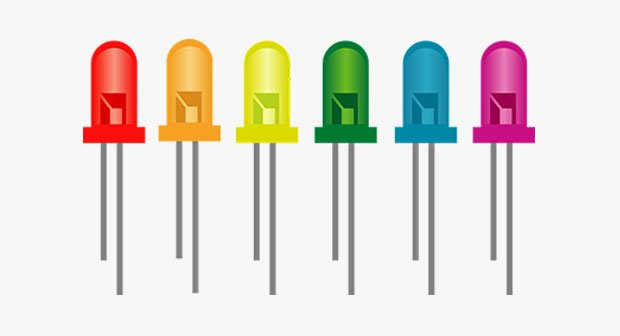
\includegraphics[width=1\textwidth]{figures/led.JPG}}
	\caption{led.}
	\label{LED}
\end{figure}

LED adalah lampu kecil (singkatan dari \"light emitting diode\") yang bekerja dengan daya yang relatif kecil. Dewan Arduino memiliki satu built-in pada pin digital 13.
Untuk mengedipkan LED hanya membutuhkan beberapa baris kode. Hal pertama yang kita lakukan adalah mendefinisikan sebuah variabel yang akan menahan jumlah pin yang 
terhubung dengan LED. Kita tidak perlu melakukan ini (kita bisa menggunakan nomor pin di seluruh kode) tapi itu membuat lebih mudah untuk mengganti pin yang berbeda. 
Kami menggunakan variabel integer (disebut int). Seperti lampu pijar dan tidak seperti kebanyakan lampu neon (misalnya tabung dan lampu neon kompak atau CFL), LED mencapai kecerahan penuh tanpa memerlukan waktu pemanasan kehidupan pencahayaan neon juga dikurangi dengan sering menyalakan dan mematikan. Biaya awal LED biasanya lebih tinggi. Degradasi pewarna LED dan bahan kemasan mengurangi keluaran cahaya sampai batas tertentu dari waktu ke waktu.
Beberapa lampu LED dibuat untuk menjadi pengganti drop-in yang kompatibel secara langsung untuk lampu pijar atau lampu neon. Kemasan lampu LED dapat menunjukkan output lumen, konsumsi daya dalam watt, suhu warna pada kelvin atau deskripsi, kisaran suhu operasi, dan kadang-kadang watt setara lampu pijar dari keluaran bercahaya serupa. Chip LED memerlukan arus listrik arus searah terkontrol (DC) dan rangkaian yang sesuai sebagai driver LED diperlukan untuk mengubah arus bolak balik dari catu daya ke arus arus yang diatur yang diatur oleh LED. LED terpengaruh oleh suhu tinggi, sehingga lampu LED biasanya mencakup elemen disipasi panas seperti heat sink dan sirip pendinginan. Driver LED adalah komponen penting lampu LED atau tokoh-tokoh. Driver LED yang baik dapat menjamin umur yang panjang untuk sistem LED dan memberikan fitur tambahan seperti peredupan dan kontrol. Driver LED dapat diletakkan di dalam lampu atau luminer, yang disebut tipe built-in, atau diletakkan di luar, yang disebut tipe independen. Menurut berbagai aplikasi, berbagai jenis driver LED perlu diterapkan, misalnya pengemudi outdoor untuk lampu jalan, pengemudi titik dalam ruangan untuk lampu bawah, dan driver linier dalam ruangan untuk lampu panel.
\subsection{Resistor}

\begin{figure}[ht]
	\centerline{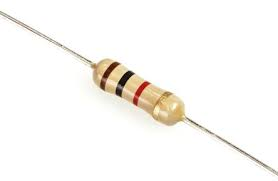
\includegraphics[width=1\textwidth]{figures/resistor.JPG}}
	\caption{resistor.}
	\label{OA:resistor}
\end{figure}
	
Sebuah resistor adalah komponen listrik dua terminal pasif yang menerapkan hambatan listrik sebagai elemen rangkaian. Di sirkuit elektronik, resistor digunakan 
untuk mengurangi arus, menyesuaikan level sinyal, membagi tegangan, elemen aktif biasa, dan menghentikan jalur transmisi, di antara kegunaan lainnya. Resistor 
berdaya tinggi yang dapat mengusir banyak daya listrik karena panas dapat digunakan sebagai bagian kontrol motor, dalam sistem distribusi tenaga, atau sebagai 
beban uji untuk generator. Resistor tetap memiliki tahanan yang hanya sedikit berubah dengan suhu, waktu atau voltase operasi. Resistor variabel dapat digunakan 
untuk mengatur elemen rangkaian (seperti kontrol volume atau lampu dimmer), atau sebagai alat penginderaan untuk panas, cahaya, kelembaban, gaya, atau aktivitas 
kimia. Resistor adalah elemen umum jaringan listrik dan sirkuit elektronik dan ada di mana-mana di peralatan elektronik. Resistor praktis sebagai komponen diskrit dapat terdiri dari berbagai senyawa dan bentuk. Resistor juga diimplementasikan dalam sirkuit terpadu.
Fungsi kelistrikan resistor ditentukan oleh resistannya: resistor komersial yang umum dibuat dengan kisaran lebih dari sembilan orde. Nilai nominal resistansi berada di dalam toleransi manufaktur, yang ditunjukkan pada komponen.
\subsection{BreadBoard}
BreadBoard adalah basis konstruksi untuk prototyping elektronik. Awalnya itu benar-benar papan roti, sepotong kayu yang dipoles yang digunakan untuk mengiris roti. Pada tahun 1970-an papan tempat memotong roti solder (a.k.a. plugboard, papan terminal terminal) tersedia dan saat ini istilah \"papan tempat memotong roti\" biasanya digunakan untuk merujuk pada ini.
Karena Breadboard solder tidak memerlukan penyolderan, itu bisa digunakan kembali. Hal ini membuat mudah digunakan untuk membuat prototipe sementara dan bereksperimen dengan desain sirkuit. Untuk alasan ini, papan roti tanpa pemanah juga sangat populer di kalangan pelajar dan dalam pendidikan teknologi. Jenis breadboard yang lebih tua tidak memiliki properti ini. Sebuah papan strip (Veroboard) dan papan sirkuit cetak prototip yang serupa, yang digunakan untuk membuat prototipe solder semi permanen atau satu kali, tidak dapat dengan mudah digunakan kembali. Berbagai sistem elektronik dapat dibuat prototip dengan menggunakan papan tempat memotong roti, dari rangkaian analog dan digital kecil hingga menyelesaikan unit pemrosesan pusat (CPU).

\subsection{Buzzer}

%\begin{figure}[ht]
%	\centerline{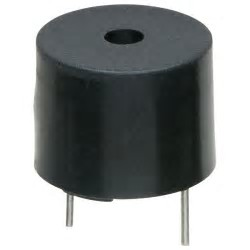
\includegraphics[width=1\textwidth]{figures/buzzer.JPG}}
%	\caption{buzzer.}
%	\label{buzzer}
%\end{figure}
	
Bel atau pager adalah perangkat sinyal audio, yang mungkin mekanis, elektromekanis, atau piezoelektrik (piezo singkatnya). Khas penggunaan buzzer dan beepers termasuk 
perangkat alarm, timer, dan konfirmasi masukan pengguna seperti klik mouse atau keystroke.

\subsection{Sejarah}
\begin{itemize}
\item Elektromekanis
Bels listrik ditemukan pada tahun 1831 oleh Joseph Henry. Mereka terutama digunakan di bel pintu awal sampai mereka berhenti di awal tahun 1930an untuk mendukung
lonceng musik, yang memiliki nada lebih lembut.
\item Piezoelektrik

%\begin{figure}[ht]
%	\centerline{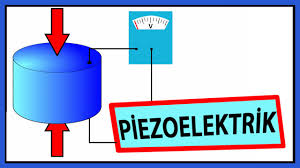
\includegraphics[width=1\textwidth]{figures/piezoelektrik.JPG}}
%	\caption{piezoelektrik.}
%	\label{piezoelektrik}
%\end{figure}
	
Cahaya piezoelektrik, atau buzz piezo, seperti yang kadang-kadang disebut, ditemukan oleh pabrikan Jepang dan dilengkapi dengan beragam produk selama tahun 1970an 
sampai 1980an. Kemajuan ini terutama terjadi karena usaha koperasi oleh perusahaan manufaktur Jepang. Pada tahun 1951, mereka mendirikan Barium Titanate Aplikasi 
Research Committee, yang memungkinkan perusahaan untuk menjadi \"kompetitif koperasi\" dan membawa beberapa inovasi piezoelektrik dan penemuan.
\end{itemize}

\subsection{Jenis-jenis Buzzer}
\begin{itemize}
\item Elektromekanis
Perangkat awal didasarkan pada sistem elektromekanis yang identik dengan bel listrik tanpa gong logam. Demikian pula, relay dapat dihubungkan untuk mengganggu 
arus penggeraknya sendiri, menyebabkan kontak buzz. Seringkali unit ini berlabuh ke dinding atau plafon untuk menggunakannya sebagai papan suara. Kata \"bel\" 
berasal dari suara serak yang dibuat oleh buzz elektromekanis.
\item Mekanis
Joy buzzer adalah contoh bel yang mekanis dan mereka memerlukan driver. Joy buzzer (juga disebut buzzer tangan) adalah perangkat lelucon praktis yang terdiri 
dari pegas melingkar di dalam disk yang dikenakan di telapak tangan. Saat pemakainya berjabat tangan dengan orang lain, sebuah tombol di cakram melepaskan 
pegas, yang dengan cepat melepaskan getaran yang terasa seperti sengatan listrik pada seseorang yang tidak mengharapkannya.

Joy buzz diciptakan pada tahun 1928 oleh Soren Sorensen Adams dari SS Adams Co. Ini dimodelkan berdasarkan produk lain, The Zapper, yang mirip dengan buzz 
belaian, namun tidak memiliki buzz yang sangat efektif dan berisi sebuah tombol yang memiliki Titik tumpul yang akan menyakiti orang yang tangannya terguncang.

Adams membawa sebuah prototipe yang agak besar dari bel yang baru dirancangnya ke Dresden, Jerman, di mana seorang masinis menciptakan alat yang akan membuat 
bagian-bagian untuk ukuran palang baru Joy Buzzer. Pada tahun 1932, item tersebut menerima Paten A.S. 1.845.735 dari Kantor Paten A.S. Keberhasilan instan dari 
barang baru tersebut memungkinkan Adams pindah ke gedung baru dan menambah ukuran perusahaannya. Adams terus mengirim pembayaran royalti ke alat dan pembuatnya 
sampai tahun 1934, saat pembayaran dikembalikan.

Pada tahun 1987, putra Sam Adams, Joseph \"Bud\" Adams, merancang ulang mekanisme untuk daya tahan yang besar dan buzz yang lebih keras, dan memasarkannya sebagai
Super Joy Buzzer.

Kesalahpahaman yang umum - terutama karena iklan palsu oleh pembuat dan penjual perangkat - adalah bahwa buzz belaka benar-benar menimbulkan kejutan listrik, 
dan banyak penjahat bergaya dalam fiksi (misalnya musuh Batman The Joker) menggunakan kegembiraan \"yang sangat kuat\" belers sebagai senjata Contohnya adalah 
dalam manga Mickey Mouse milik Walt Disney Mickey's Mouse dimana tangan Mickey Mouse terguncang oleh celana Celana Mortimer. Contoh lain adalah di episode 
SpongeBob SquarePants \"Pranks a Lot\" di mana tangan Patrick Star dikejutkan oleh buzz gembira, dan dalam episode The Simpsons \"Homer the Clown\", di mana Homer 
Simpson dikejutkan berkali-kali oleh Krusty the Clown to the titik dimana dia disiksa olehnya. Namun, pena yang mengejutkan memang menghasilkan sengatan listrik
ringan saat korban menekan tombol di atas; pena bisa diputar untuk membuatnya melepaskan intinya.

Contoh lain dari mereka adalah bel pintu.
\item Piezoelektrik
Piezoelektrik / piˌeɪzoʊˌilɛktrɪsɪti / adalah muatan listrik yang terakumulasi pada bahan padat tertentu (seperti kristal, keramik tertentu, dan bahan biologis 
seperti tulang, DNA dan berbagai protein) [1] sebagai respons terhadap tekanan mekanis yang diterapkan. Kata piezoelektrik berarti listrik akibat tekanan dan 
panas laten. Ini berasal dari piezein πιέζειν Yunani, yang berarti meremas atau menekan, dan ἤλεκτρον ēlektron, yang berarti amber, sumber muatan listrik kuno.
[2] [3] Piezoelektrik ditemukan pada tahun 1880 oleh fisikawan Prancis Jacques dan Pierre Curie. [4]

Efek piezoelektrik dipahami sebagai interaksi elektromekanis linier antara keadaan mekanis dan listrik pada bahan kristal tanpa simetri inversi.

Piezoelektrik ditemukan pada aplikasi yang berguna, seperti produksi dan pendeteksian suara, generasi tegangan tinggi, generasi frekuensi elektronik, mikrobalances, 
untuk menggerakkan nosel ultrasonik, dan ultrafine yang memfokuskan pada majelis optik. Ini juga merupakan dasar dari sejumlah teknik instrumental ilmiah dengan 
resolusi atom, mikroskop probe pemindaian, seperti STM, AFM, MTA, SNOM, dll., Dan penggunaan sehari-hari, seperti bertindak sebagai sumber pengapian untuk pemantik 
api, dan barbeque propana push-start, serta sumber referensi waktu pada jam tangan kuarsa.

Piezoelectric disk beeper
Elemen piezoelektrik dapat didorong oleh sirkuit elektronik berosilasi atau sumber sinyal audio lainnya, yang digerakkan dengan amplifier audio piezoelektrik. Kedengarannya biasa digunakan untuk menunjukkan bahwa tombol yang telah ditekan adalah klik, sebuah cincin atau bunyi bip.

Bagian dalam bel yang readymade, menunjukkan puster piezoelektrik (Dengan 3 elektroda ... termasuk 1 elektroda umpan balik (elektroda kecil dan pusat yang digabungkan dengan kawat merah di foto ini), dan osilator untuk menggerakkan bel sendiri.
Sebuah buzzer piezoelektrik / pager juga tergantung pada resonansi rongga akustik atau resonansi Helmholtz untuk menghasilkan bunyi bip yang terdengar.
\end{itemize}

\cite{series1994atlas}
